\newpage
\appendix
\section {Proofs.}

\begin {framed}
{\bf Theorem 1.}
	\[p_{nf}^{cel}=\P\left[SNR_{nf}\ge\Theta_b\right]=\P\left[d\le R_1\right]=1-\P\left[d>R_1\right]=1-\P\left[\Phi_b(A)=0\right]\]
	\[=1-e^{-\lambda_b\pi R_1^2}\]
where \(A\) is the area of search disk of radius \(R_1\).
\end {framed}

\begin {framed}
{\bf Theorem 2.}
    \par The scenario of getting connectivity by means of a D2D relay is represented by event $C=A\cap B$, where event $A$ is $R_1<d\le R_1+R_2$; and event $B$ represents the existence of at least 1 user in the area of $b(O,R_2)\cap b(B_{nst},R_1)$ - let us denote this area as $D$.
	\par More precisely, the following probability is considered:
	$$\P[C]=\P[A\cap B]=$$
	\begin{equation}
	    \P\left[(R_1<d\le R_1+R_2)\cap (\Phi_u(D(d)))\ge 1\right]
	\end{equation}
	\par Here, $d$ is a random variable. And consequently, the area of $D$ depends on the value of $d$.
	\par Consider $f_d(r)$ - probability density function of the random variable $d$:
	$$f_d(r)=\frac{d}{dr}F_d(r)=\frac{d}{dr}\left(\P(d\le r)\right)$$
	$$=\frac{d}{dr}\left(1-\P(d>r)\right)=\frac{d}{dr}\left(1-\P(\Phi_b(b(O,r))=0)\right)$$
	$$=\frac{d}{dr}\left(1-e^{-\lambda_b\pi r^2}\right)=2\lambda_b\pi re^{-\lambda_b\pi r^2}$$
	\par Here, $F_d(r)$ is a cumulative distribution function of the random variable $d$.
	\par Interpreting (1) in terms of (4), denoting event $A$ as ${\Phi_u(D(d))\ge1}$, and subset $B=(R_1;R_1+R_2]$:
	$$\P\Big[(R_1<d\le R_1+R_2)\cap (\Phi_u(D(d))\ge 1)\Big]$$
	$$=\P({\Phi_u(D(d))\ge1},d\in (R_1;R_1+R_2])$$
	$$=\int_{(R_1;R_1+R_2]}f_d(r)\P\Big(\Phi_u(D(d)\ge1)\Big|d=r\Big)dr$$
	$$=\int_{(R_1;R_1+R_2]}f_d(r)\P(\Phi_u(D(r))\ge1)dr$$
	$$=\int_{(R_1;R_1+R_2]}f_d(r)\big(1-\P(\Phi_u(D(r))=0)\big)dr$$
	\begin{equation}
	    =\int_{(R_1;R_1+R_2]}2\lambda_b\pi re^{-\lambda_b\pi r^2}\Big(1-e^{-\lambda_u|D(r)|}\Big)dr
	\end{equation}
	where
	$$|D(r)|=R_2^2\cos^{-1}\Big(\frac{r^2+R_2^2-R_1^2}{2rR_2}\Big)+R_1^2\cos^{-1}\Big(\frac{r^2+R_1^2-R_2^2}{2rR_1}\Big)$$
	$$-\frac{1}{2}\sqrt{(-r+R_2+R_1)(r+R_2-R_1)(r-R_2+R_1)(r+R_1+R_2)}$$
\end {framed}

\begin {framed}
{\bf Theorem 4.}
Conditioning on the nearest base station being at a distance $r$ from a typical user:
	$$p_c = \P\big[SNR\ge\Theta_b\big| d=r\big]$$
	$$= \P\Big[\frac{P_bhd^{-\beta_b}}{N_b}\ge\Theta_b\Big|d=r\Big]$$
	$$= \int_{r>0}\P\Bigg[h\ge\frac{\Theta_b N_b r^{\beta_b}}{P_b}\Bigg]f_d(r)dr$$
	$$= 2\lambda_b\pi\int_{r>0}e^{-\frac{\mu\Theta_b N_b r^{\beta_b}}{P_b}}re^{-\lambda_b\pi r^2}dr$$
\end {framed}

\section {Plots.}
{\bf Picture 1.}
\\
    \begin{tikzpicture}[scale=.5]
        \begin{axis}[
            xmin=-3,xmax=3,
            ymin=-3,ymax=3,
            extra x ticks={-1,1,-2,2,-3,3},
            extra y ticks={-1,1,-2,2,-3,3},
            extra tick style={grid=both},
        ]
        \draw[red] \pgfextra{
          \pgfpathcircle{\pgfplotspointaxisxy{0}{0}}{2.5cm}
          };
        \node[inner sep=0pt] (receiver) at (3.4cm,2.9cm)
            {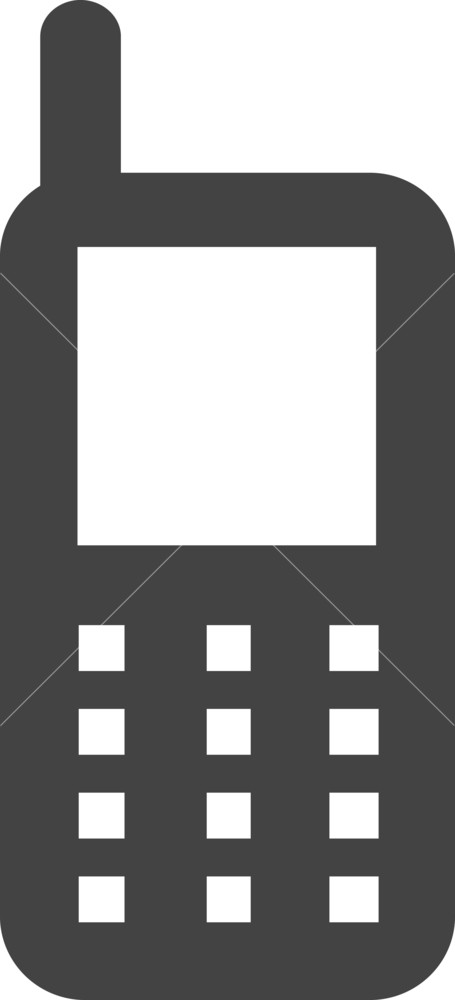
\includegraphics[width=.1\textwidth]{phone.jpg}};
        \node[inner sep=0pt] (receiver) at (4.4cm,0.9cm)
            {
\includegraphics[width=.3\textwidth]{bs.png}};
        \end{axis}
    \end{tikzpicture}

\\{\bf Picture 2.}
\\
    \begin{tikzpicture}[scale=0.5]
        \begin{axis}[
            xmin=-3,xmax=10,
            ymin=-3,ymax=10,
            extra x ticks={0,-1,1,-2,2,-3,3,-4,4},
            extra y ticks={0,-1,1,-2,2,-3,3,-4,4},
            extra tick style={axis equal=true,grid=both},
        ]
		\draw[red,dashed] \pgfextra{
		  \pgfpathcircle{\pgfplotspointaxisxy{0}{0}}{2.5cm}
		};
		\draw[red,dashed] \pgfextra{
		  \pgfpathcircle{\pgfplotspointaxisxy{4}{4}}{2.5cm}
		};
		\draw[blue] \pgfextra{
		  \pgfpathcircle{\pgfplotspointaxisxy{0}{0}}{1cm}
		};
		\addplot graphics[xmin=-0.2,xmax=0.2,ymin=-0.4,ymax=0.4]{phone.jpg};
		\addplot graphics[xmin=0.8,xmax=1.2,ymin=0.6,ymax=1.4]{phone.jpg};
		\addplot graphics[xmin=3.6,xmax=4.4,ymin=3.6,ymax=4.6]{bs.png};
        \end{axis}
    \end{tikzpicture}

%\\
%\\{\bf Search area for \(90^{\circ}\) and \(180^{\circ}\)}
%\\
%\begin{figure}[h]
  \centering
  \begin{minipage}{.2\linewidth}
    \centering
    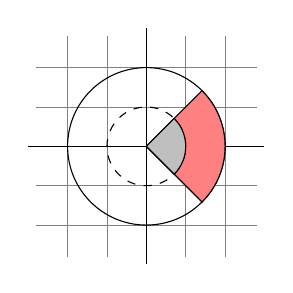
\begin{tikzpicture}
      \draw[step=.5cm,gray,very thin] (-1.4,-1.4) grid (1.4,1.4);
      \draw (-1.5,0) -- (1.5,0);
      \draw (0,-1.5) -- (0,1.5);
      \draw (0,0) circle (1cm);
      \draw[fill=red!50] (0,0) -- +(-45:1cm)
      arc (-45:45:1cm) -- cycle;
      \draw [dashed] (0,0) circle (.5cm);
      \draw[fill=gray!50] (0,0) -- +(-45:.5cm)
      arc (-45:45:.5cm) -- cycle;
    \end{tikzpicture}
  \end{minipage}\hspace{3cm}
  \begin{minipage}{.2\linewidth}
    \centering
    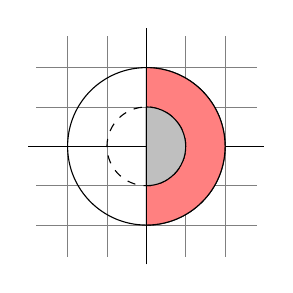
\begin{tikzpicture}
      \draw[step=.5cm,gray,very thin] (-1.4,-1.4) grid (1.4,1.4);
      \draw (-1.5,0) -- (1.5,0);
      \draw (0,-1.5) -- (0,1.5);
      \draw (0,0) circle (1cm);
      \draw[fill=red!50] (0,0) -- +(-90:1cm)
      arc (-90:90:1cm) -- cycle;
      \draw [dashed] (0,0) circle (.5cm);
      \draw[fill=gray!50] (0,0) -- +(-90:.5cm)
      arc (-90:90:.5cm) -- cycle;
    \end{tikzpicture}
  \end{minipage}
\end{figure}


\begin{comment}
\section {Geometry of the area of search of a relay node in D2D multiple relay links scenario}
As we consider two circles, one inside the other, of some radiuses \(R_1=R\) and \(R_2=R_1/2\), let's focus on two circular sectors. Let's denote the areas of the bigger and smaller sectors as \(S_{sect_1}\text{ and }S_{sect_2}\); the areas of the bigger and smaller triangle portions of the sectors as \(S_1\text{ and }S_2\) respectively; the circular segments of the bigger and smaller sectors as \(S_3\text{ and }S_4\) respectively; and the area of a trapezium formed with the bases of the smaller and the bigger triangles as \(S_{trap}\).
\\ Then, the necessary area for the search would be expressed as:
\[S_{search}=(S_{trap}-S_4)+(S_{sect}-S_1)\]
We focus on three values for the central angle: \(\alpha = {45^{\circ}, 90^{\circ}, 180^{\circ}}\) for easier calculations. We use the next formulas of the areas:
\[S_{sect_{1,2}}=\frac{1}{2}R_{1,2}^2\theta\text{ , area of the sector where }\theta\text{ is the central angle value in radians}\]
\[S_{1,2}=\frac{1}{2}ab\sin{\alpha}\text{, where }a\text{ and }b\text{ are the respective radiuses of the circles}\]
\[S_3=S_{sect_1}-S_1\text{, }S_4=S_{sect_2}-S_2\]
As for the bases of the bigger and smaller triangles, we apply the law of cosines:
\[a_{1,2}=\sqrt{2R_{1,2}^2-2{R_{1,2}^2\cos{\alpha}}}\]
\[S_{trap}=\frac{1}{2}h(a+b)=\frac{1}{2}\Big(\frac{2S_1}{a_1}-\frac{2S_2}{a_2}\Big)(a+b)\]
The following table displays the results for each value of the central angle:
\begin{table}[h!]
  \centering
	\begin{tabular}{c|c|c|c|}
	 & \(45^{\circ}\) & \(90^{\circ}\) & \(180^{\circ}\) \\ [1ex]
	\(S_{search}\) & & \(\frac{1}{16}(3\pi+6)R^2\) &  \\ [1ex]
	\end{tabular}
\end{table}
\par But this approach is not actual since the focus is on a coridor of search. Based upon the analytical form of a circle with radius \(a\):
\[x^2+y^2=a^2\]
we formulate the parameter constraints for the central angle being equal to \(90^{\circ}\) and \(180^{\circ}\). Namely:
\[x^2+y^2=R_2^2\text{ , }0\le x\le R_2\text{, }-x\le y\le x\]
\[x^2+y^2=R_2^2\text{ , }0\le x\le R_2\text{, }-R_2\le y\le R_2\]
respectively.
In terms of integration, it will be expressed as:
\[A_{90}(a,b)=\int_{-x}^{x}\int_{a}^{b}\big(x^2+y^2\big)dxdy=\int_{a}^{b}\Big(x^2\int_{-x}^{x}dy+\int_{-x}^{x}y^2dy\Big)dx\]
\begin{equation}
=\frac{8}{3}\int_{a}^{b}x^{3}dx=\frac{2}{3}\Big(b^4-a^4\Big)
\end{equation}
for \(90^{\circ}\), and:
\[A_{180}(a,b)=\int_{-R_2}^{R_2}\int_{a}^{b}\big(x^2+y^2\big)dxdy=\int_{-R_2}^{R_2}\Big(\int_{a}^{b}x^2dx+y^2\int_{a}^{b}dx\Big)dy\]
\begin{equation}
=\int_{-R_2}^{R_2}\Big(\frac{1}{3}\big(b^3-a^3\big)+y^2(b-a)\Big)dy=\frac{2}{3}R_2\big(b^3-a^3+R_2^2(b-a)\big)
\end{equation}
\end{comment}
